

\def\figw{8cm}
\def\figh{5cm}


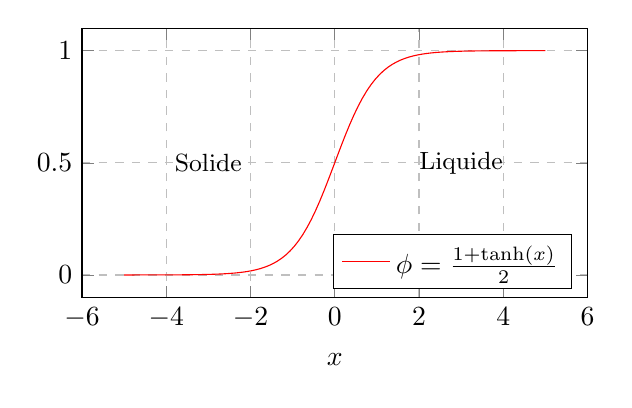
\begin{tikzpicture}
\begin{axis}[
% title=(a) Indicatrice diffuse,
%axis lines = left,
xlabel = \(x\vphantom{\phi}\),
% ylabel = {\(\phi\)},
xmajorgrids=true,
ymajorgrids=true,
grid style=dashed,
legend pos=south east,
width=\figw,
height=\figh,
ymin=-0.1, ymax=1.1,
] % end axis options
\addplot[
domain=-5:5,
samples=100,
color=red, 
]% end plot options
{(1+tanh(\x))/2}; % end plot func
\addlegendentry{\(\phi=\frac{1+\tanh(x)}{2}\)}

\pgfplotsset{
    after end axis/.code={
        \node[] at (axis cs:3,0.5){\small{Liquide}};
        \node[] at (axis cs:-3,0.5){\small{Solide}};
    }
}
    
\end{axis}
\end{tikzpicture}


\begin{tikzpicture}
\begin{axis}[
% title=(b) Double-puits,
%axis lines = left,
xlabel = \(\phi\),
% ylabel = {\(\)},
xmajorgrids=true,
ymajorgrids=true,
grid style=dashed,
width=\figw,
height=\figh,
ymin=-0.1, ymax=1.1,
] % end axis options
\addplot[
domain=-0.3:1.3,
samples=100,
color=red, 
]% end plot options
{8*x*x*(1-x)*(1-x)}; % end plot func
\addlegendentry{\(g_{dw}(\phi)=8\phi^2(1-\phi)^2\)}
\end{axis}
\end{tikzpicture}


